%!TEX root = ../chapter1.tex
%******************************
%	 Results 
%*****************************

\section{scRNAseq of murine CD4$^+$ T cells}
\subsection*{Single-cell RNA sequencing of CD4$^+$ T cells during activation, ageing and across two mouse species}

\begin{wrapfigure}{r}{0.5\textwidth}
\centering    
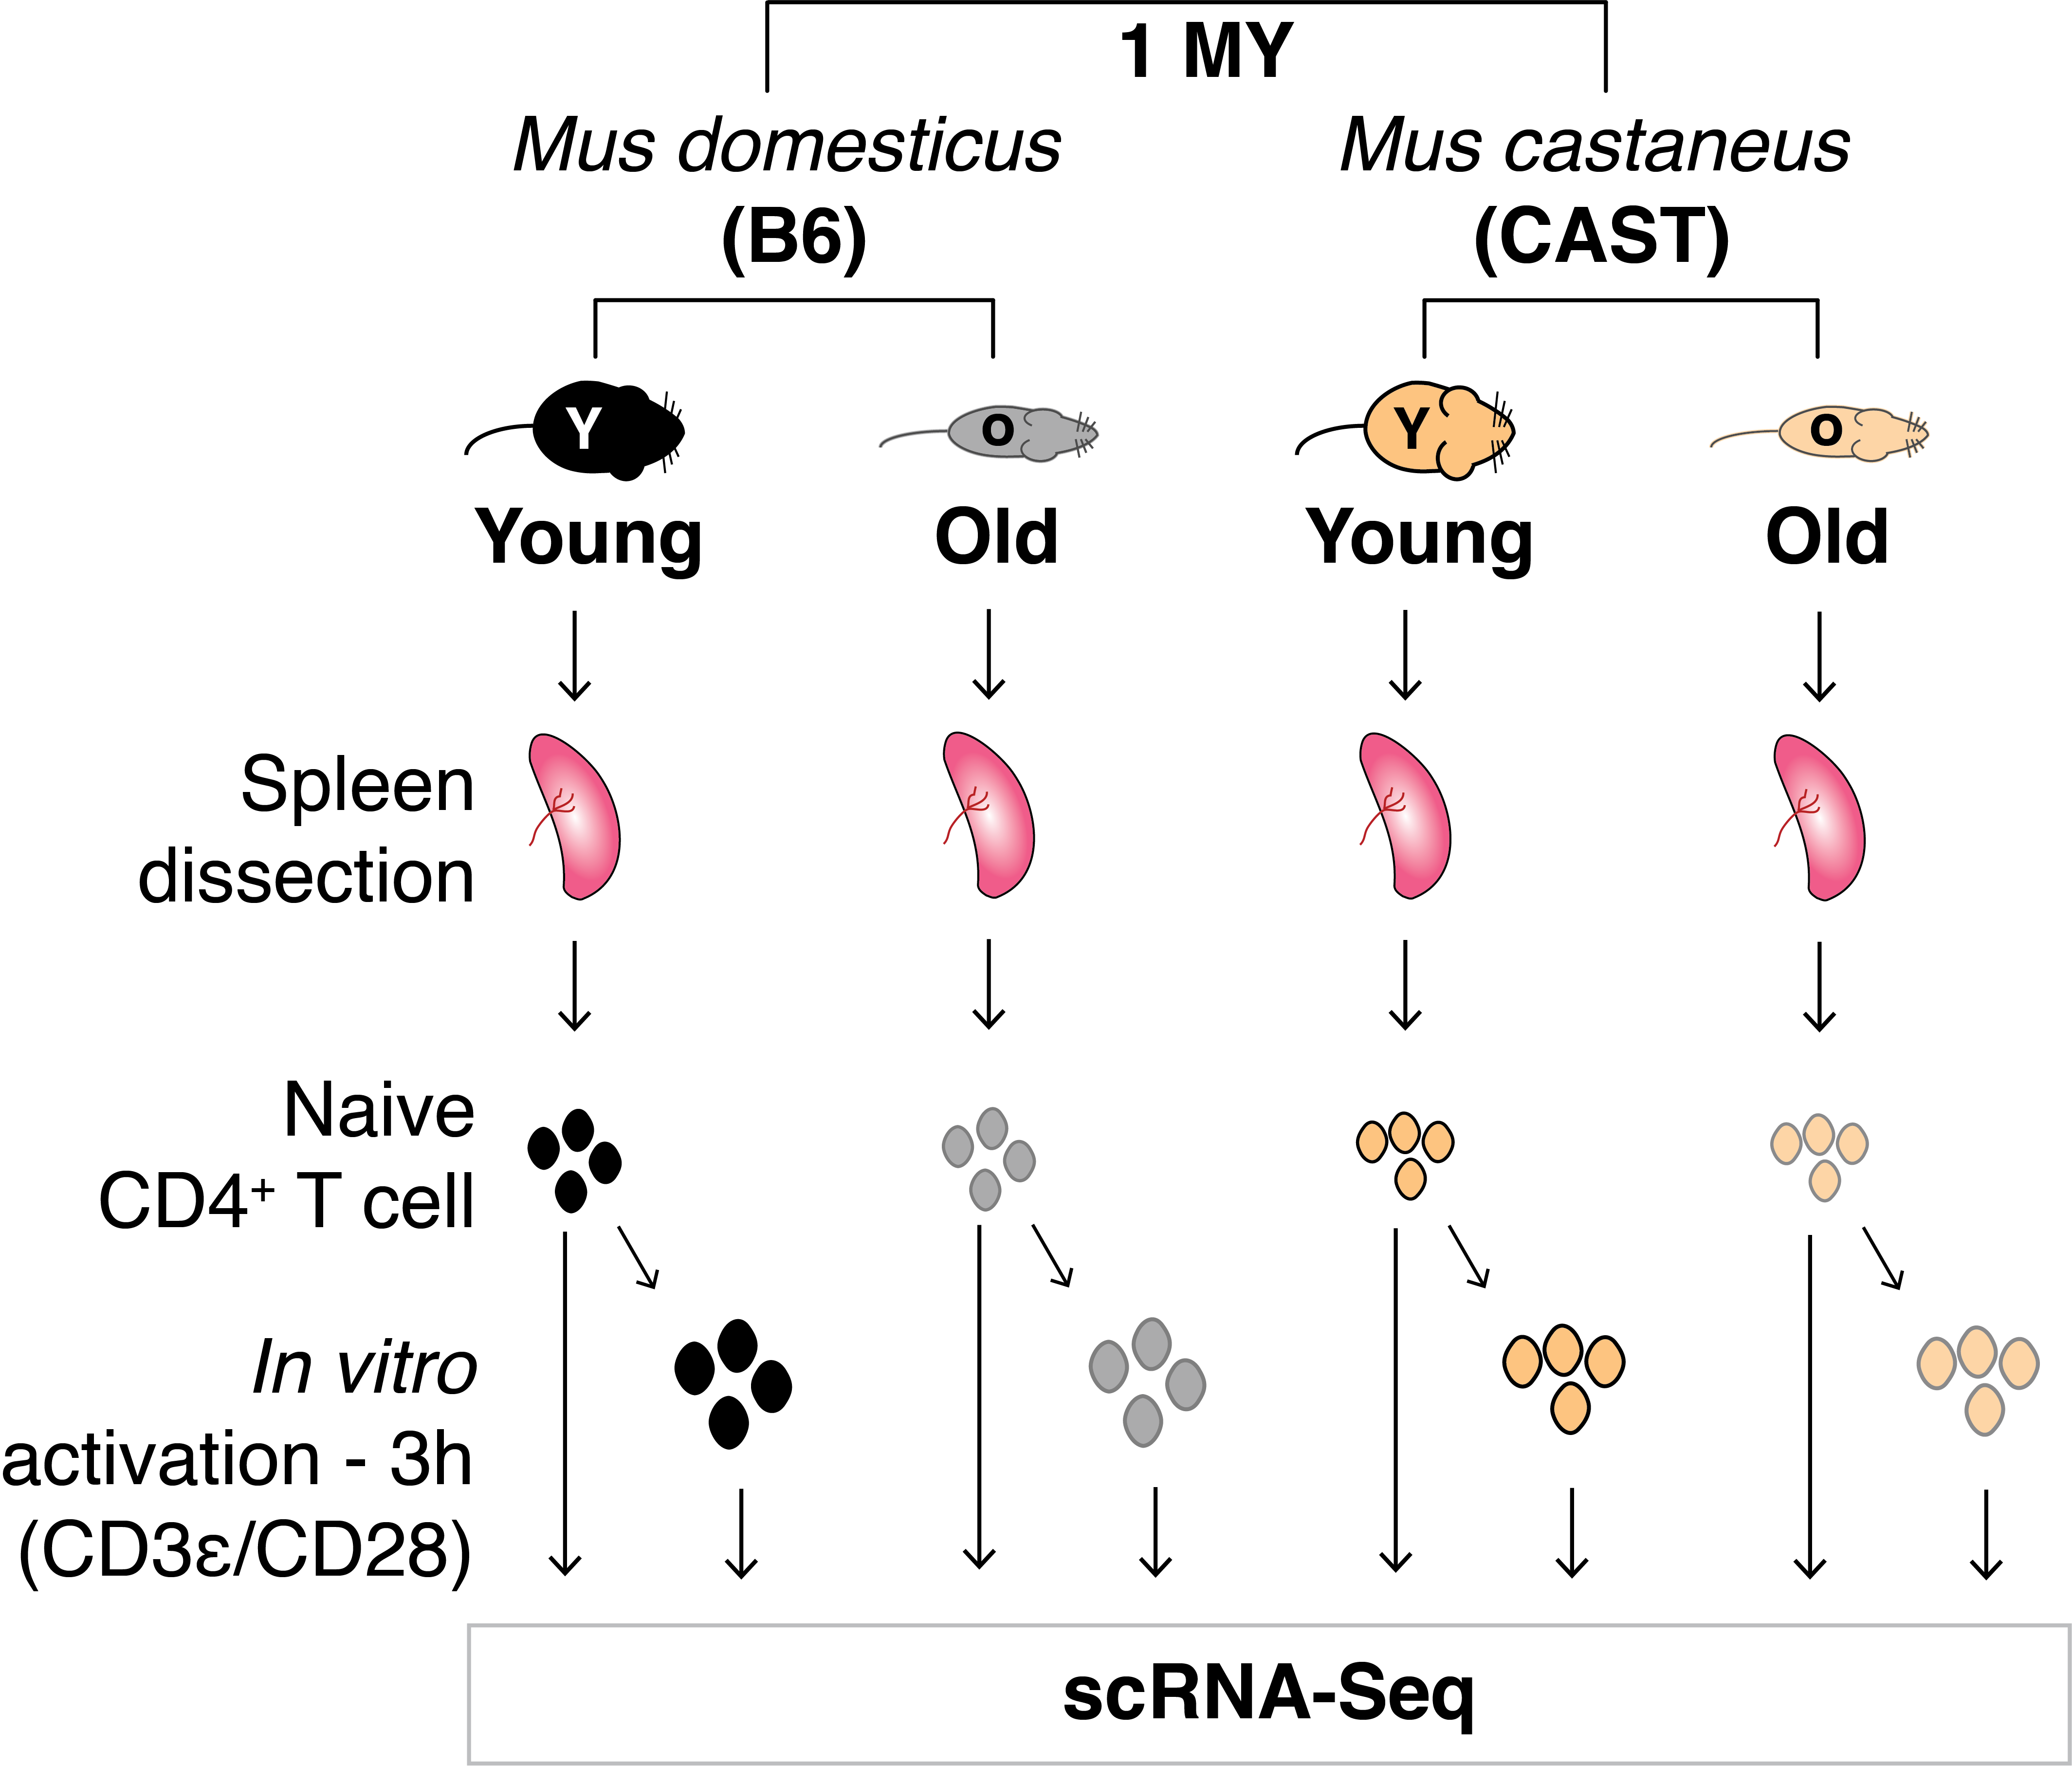
\includegraphics[width=0.48\textwidth]{Fig_1.png}
\caption[scRNAseq of CD4$^+$ T cells from young and old mice.]{\textbf{scRNAseq of unstimulated and activated CD4$^+$ T cells from young and old B6 and CAST animals.} \\
Single cells were isolated from spleens of young (~3 month) and old (~21 month) individuals of two related mouse sub-species (Mus musculus domesticus, B6; Mus musculus castaneus, CAST). Isolated cells were subjected to single-cell mRNA sequencing (scRNAseq) before or after 3 hours of in vitro activation using anti-CD3$\epsilon$/CD28 coated plates.}
\label{fig:chapt1_overview}
\end{wrapfigure}

To assess the conservation of immune activation programmes, we isolated CD4$^+$ T cells from healthy individuals of two inbred mouse sub-species separated by 1 million years of divergence: the reference C57BL/6J, Mus musculus domesticus (B6); CAST/EiJ, Mus musculus castaneus (CAST)). We characterized their gene expression programmes by single-cell RNA-sequencing (scRNAseq) during ageing in young (~3 months) and old (~21 months) individuals of each strain \textbf{(Fig. \ref{fig:chapt1_overview})}. These two sub-species have similar lifespans \citep{Yuan2011}, and CAST mice showed the hallmarks of normal organismal aging observed in B6 mice \citep{Rodwell2004}. All mice were healthy at the time of experiments. To asses different CD4$^+$ T cell compartments, we assayed cell populations with different levels of purity. First, we isolated all unstimulated CD4$^+$ T cells from spleen of old and young animals. Secondly, we highly purified naive CD4$^+$ T cells and effector memory (EM) CD4$^+$ T cells. For each species/condition, scRNA-seq experiments were performed using cells isolated from two individual mice.

\subsubsection*{Unstimualted CD4$^+$ T cells}

Unstimulated naive CD4$^+$ T cells were purified from dissociated mouse spleens using cell strainers, cell separation media and a CD4$^+$ CD62L$^+$ T Cell Isolation Kit. Purified naive CD4$^+$ T cells were cultured in IMDM medium supplemented with 10\% Fetal Bovine Serum, 1 $\mu$g/mL Penicillin/Streptomicin, and 50 $\mu$M 2-mercaptoethanol. \\

\subsubsection{Naive and effector memory CD4$^+$ T cells}

\begin{wrapfigure}{r}{0.5\textwidth}
\centering    
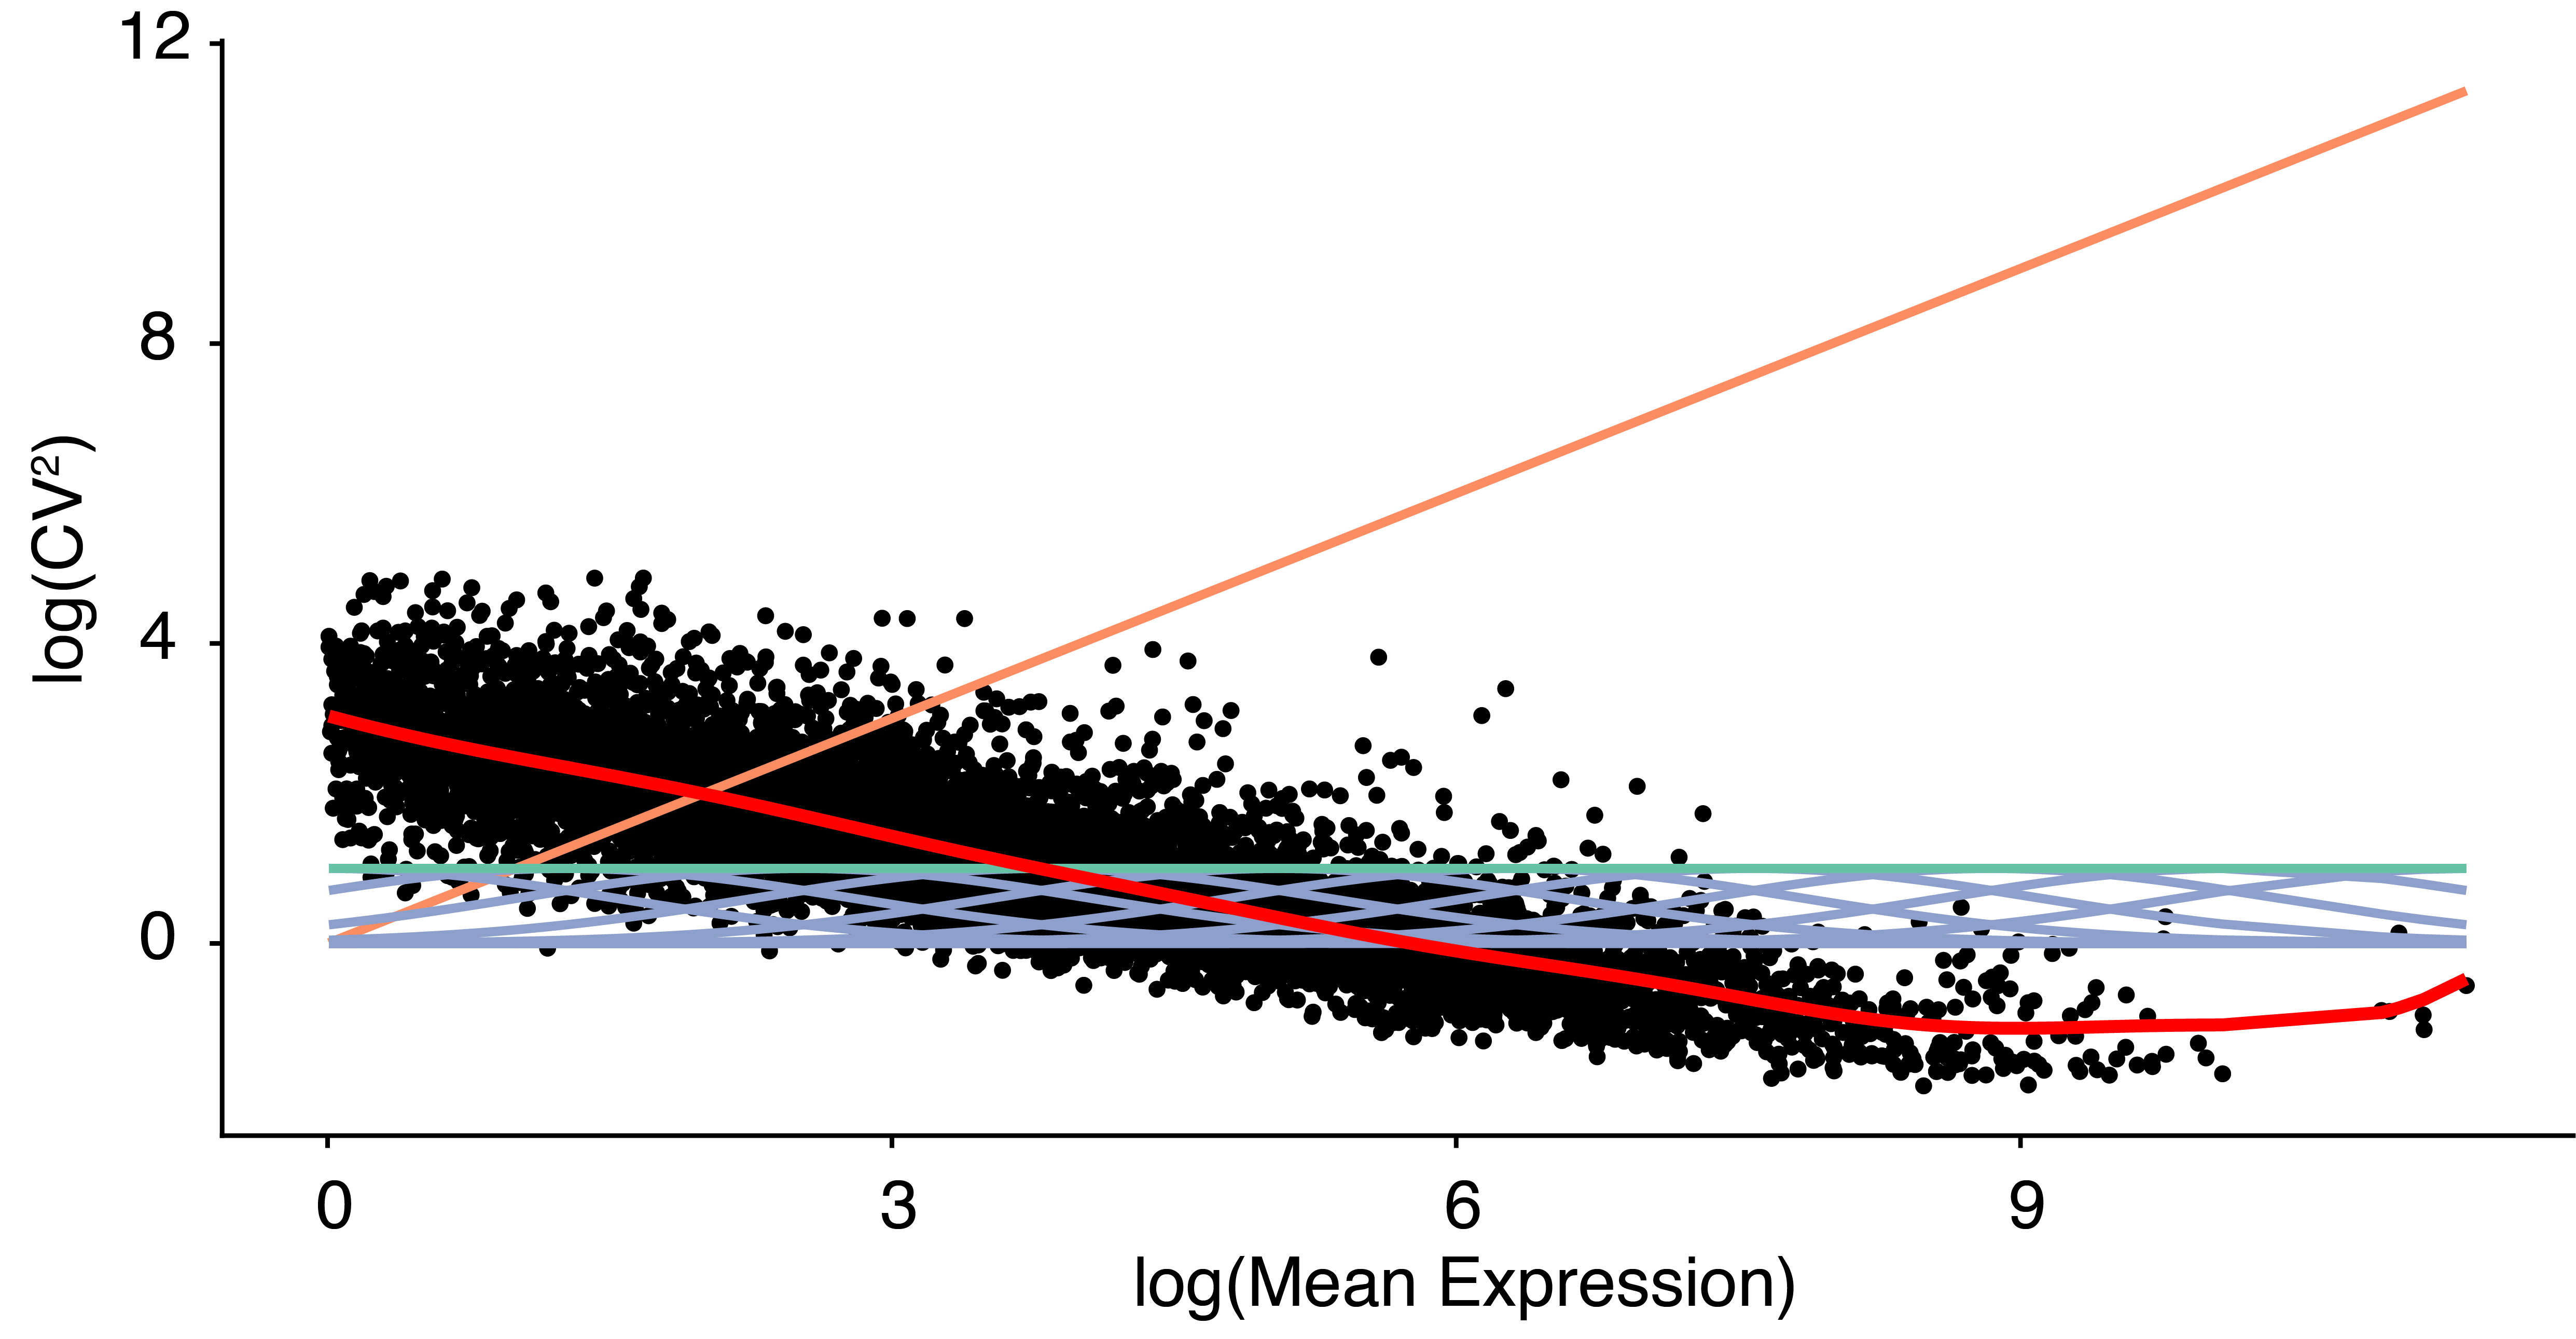
\includegraphics[width=0.48\textwidth]{Fig_2.png}
\caption[FACS of naive and effector mempry CD4$^+$ T cells.]{\textbf{FACS of naive and effector mempry CD4$^+$ T cells.} \\
Gating Strategy: lymphocytes were gated by the use of forward scatter (FSC-A) and side scatter (SSC-A). Cell doublets were excluded according to area and height of forward scatter (FSC-A/FSC-H). Dead cells were removed using viability dye. PD-1$^+$ CD4$^+$ T cells were excluded and PD-1-ve CD4$^+$ T cells were further separated into naive and EM CD4$^+$ T cell subsets according to their CD44 and CD62L expression. Cells with a mature CD24lo Qa2hi phenotype were then gated from naive and EM subsets and CD69+ cells were removed.}
\label{fig:FACS}
\vspace*{-20mm}
\end{wrapfigure}

Naive and effector memory CD4$^+$ T cells were purified from spleens of both young and old C57/BL6 mice by FACS.  Briefly, spleens were harvested from both young and old animals and single cell suspensions were obtained by meshing through a cell strainer (70 $\mu$m). B cells were depleted from cell suspensions by MACS using CD19 microbeads and red blood cells were lysed with RBC lysis buffer. The enriched cell fraction was then stained with Fixable eFluor 780 viability dye following by Fc receptor blocking with TruStain fcXTM and subsequent staining with a panel of fluorescence-conjugated antibodies against CD4, CD44, CD62L, CD24, Qa2, CD69 and PD-1.  Stained cells were immediately sorted using a 5-laser Aria IIu SORP instrument with the stringent gating strategy described in \textbf{Fig. \ref{fig:FACS}}. \\
Hereafter, for simplification and clarity, purified unstimulated CD4$^+$ T cells will be named naive, stimulated cells will be named activated.

\subsubsection*{Activation of CD4$^+$ T cells}

Naive cells were seeded into 96-well plates coated for 1h at 37ºC with anti-CD3$\epsilon$ (1 $\mu$g/ml) and anti-CD28 (3 $\mu$g/ml) at a density of 80,000-120,000 cells/ml, and then cultured in a total volume of 100 $\mu$l media that did not contain cytokines or additional antibodies.

\subsubsection*{scRNAseq using the Fluidigm C1 system}

Naive, purified naive and activated CD4+ T cells were immediately collected and loaded on a 5–10$\mu$m Auto Prep Integrated Fluidic Circuit (IFC) to capture single cells using the C1 Single cell Auto Prep System (Fluidigm). All IFCs were visually inspected, and wells with multiple cells or cell debris were marked as low quality. Upon cell capture, reverse transcription and cDNA amplification were performed using the SMARTer PCR cDNA Synthesis Kit and the Advantage 2 PCR Kit. ERCC spike-in RNA (1 $\mu$L diluted at 1:50,000) was added to the C1 lysis mix. All capture sites were included for the RNA-seq library preparation.

\subsubsection*{Computational quality control and filtering}

We visually inspected the vast majority of cell-capture sites in each C1 small-integrated fluidic circuit (IFCs, 5-10$\mu$m) using 40x magnification lensing to ensure precise capture of single cells (Fig. S1A and S1B and Material and Methods). We removed low-quality C1 captured cells by evaluating (i) the sequencing depth, (ii) the number of genes detected, (iii) the proportion of sequencing reads mapping to exons and ERCC controls, and (iv) the mitochondrial fraction of reads (Fig. S1C-F). The resulting data showed minimal batch effects (Fig. S1G). Using RNA-sequencing to identify cell-specific marker genes, we removed residual B-cells, CD8+ T cells, and (in activating conditions) non-activated T cells from our analysis (Fig. S1H and S1I, Material and Methods). \\

In contrast to haematopoeitic cells (15), even when activated, virtually all CD4+ T cells are in G1 phase of cell cycle as expected (Fig. S2A). Aged CD4+ T cells showed no clonal expansions (Fig. S2B) or difference in cell size (Fig. S2C) that could impact analysis of gene expression variability (26). Using flow cytometry analysis, we confirmed that 96.4\% of the isolated CD4+ T cells were naive in young B6 (Fig. S2D). Naive CD4+ T cells formed a single, high-purity population in young animals. Old animals had a small population of CD4+ T cells with slightly elevated CD44 levels, reduced CD62L expression, and attenuated activation dynamics (Fig. S2E-G); their removal did not impact our results (Material and Methods) (see below). Upon T cell receptor (TCR) activation in the presence of particular cytokines, naive CD4+ T cells can differentiate into several lineages of functionally different T helper cells (mainly Th1, Th2, Th17, Treg, Tfh) (16, 27). In our data we do not detect any early differentiation in naive and activated CD4+ T cell subsets. In accordance with the literature we found Gata3 but not Th2 cytokines expressed in the majority of cells  (28). Interestingly, the Th1-related genes Tbx21 and Ifng were up-regulated, in an uncoordinated manner, in a small population of activated CD4+ T cells of old animals. This is consistent with a known Th1 bias in CD4+ T cell responses in old mice (29) and humans (30) (Fig. S2H). Furthermore, we did not detect any difference in TCR components/signaling and importantly detected no signs of T cell exhaustion (31), especially in cells isolated from old animals (Fig. S2I). We also ruled out species-specific differences in commitment towards T helper cell lineages (Fig. S2J). \\

After the above analyses and the experimental validation (Material and Methods), a total of 1514 high-quality CD4+ T cell transcriptomes were analyzed across all conditions and species.

